%
\documentclass[11pt]{article}
\usepackage{amsmath,amssymb,amsthm}
\usepackage[utf8]{inputenc}
\usepackage{graphicx}
\usepackage{xcolor}
\usepackage{hyperref}
\usepackage{algorithm,algorithmic}
\usepackage[usenames,dvipsnames,svgnames,table]{xcolor}

\DeclareMathOperator*{\E}{\mathbb{E}}
\let\Pr\relax
\DeclareMathOperator*{\Pr}{\mathbb{P}}

\newcommand{\eps}{\varepsilon}
\newcommand{\inprod}[1]{\left\langle #1 \right\rangle}
\newcommand{\R}{\mathbb{R}}


\newcommand{\handout}[5]{
	\noindent
	\begin{center}
		\framebox{
			\vbox{
				\hbox to 6.38in { \textcolor{black}{\bf CS 134: Networks } \hfill #4  }
				\vspace{1mm}
				\hbox to 6.42in { #3 {\hfill #2 } }
				\vspace{0.0mm}
				\hbox to 6.38in { { \hfill} }
			}
		}
	\end{center}
	\vspace*{0mm}
}

\newcommand{\pset}[3]{\handout{{#1}}{\textcolor{red}{Due: #2}}{\textcolor{black}{#3}}{\textcolor{gray}{\textbf{Problem set #1}}}}

\newtheorem{theorem}{Theorem}
\newtheorem{corollary}[theorem]{Corollary}
\newtheorem{lemma}[theorem]{Lemma}
\newtheorem{observation}[theorem]{Observation}
\newtheorem{proposition}[theorem]{Proposition}
\newtheorem{definition}[theorem]{Definition}
\newtheorem{claim}[theorem]{Claim}
\newtheorem{fact}[theorem]{Fact}
\newtheorem{assumption}[theorem]{Assumption}
\newtheorem{remark}[theorem]{Remark}

\newtheorem*{theorem*}{Theorem}
\newtheorem*{notation*}{Notation}
\newtheorem*{assumption*}{Assumption}
\newtheorem*{fact*}{Fact}
\newtheorem*{claim*}{Claim}
\newtheorem*{definition*}{Definition}
\newtheorem*{exercise*}{Exercise}
\newtheorem*{lemma*}{Lemma}
\newtheorem*{remark*}{Remark}

% 1-inch margins, from fullpage.sty by H.Partl, Version 2, Dec. 15, 1988.
\topmargin 0pt
\advance \topmargin by -\headheight
\advance \topmargin by -\headsep
\textheight 8.9in
\oddsidemargin 0pt
\evensidemargin \oddsidemargin
\marginparwidth 0.5in
\textwidth 6.5in

\parindent 0in
\parskip 1.5ex


\usepackage[margin=.9in]{geometry}
\usepackage{amsmath}
\usepackage{tikz}
\usepackage{float}
\usepackage{filecontents}
\usepackage{pgfplots, pgfplotstable}
%\usepgfplotslibrary{statistics}
\usepackage[T1]{fontenc}
\usetikzlibrary{calc,intersections,through,backgrounds,shadings}
\usetikzlibrary{shapes.geometric}
\usetikzlibrary{through}

\usepackage[nofiglist,nomarkers]{endfloat}
\renewcommand{\efloatseparator}{\mbox{}}

\usepackage{exercise}
\renewcommand{\ExerciseHeader}{{ \textbf{
			\ExerciseName \ \ExerciseHeaderNB \ExerciseHeaderTitle
			\ExerciseHeaderOrigin.}}}

\usepackage{pgfplots}
\pgfplotsset{
	%  compatgraph=newest,
	xlabel near ticks,
	ylabel near ticks
}


\begin{document}
	
	\pset{8}{\textbf{Wednesday 4/5/2017}}{{Prof.\ Yaron Singer}}	
	%\section*{PSET}


\paragraph{1. Alternative Definition for Submodular Functions (15 points)}
Recall that in class we said that a set function $f:2^V \to \mathbb{R}$ is \emph{submodular} if for every $S,T \subseteq V$ for which $S \subseteq T$ and $a\notin T$ we have that: 
%
$$f(S \cup a) - f(S) \geq f(T \cup a) - f(T) $$
%
\begin{itemize}
\item[\textbf{a. }] \textbf{(7 points)} Show that $f$ is a submodular function \textbf{if and only if} (iff) for every $A,B \subseteq V$ we have that: 
%
$$f(A \cup B) \leq f(A) + f(B) - f(A\cap B)$$
%
As a reminder, $A$ iff $B$ if both $A$ implies $B$ and $B$ implies $A$. 
\item[\textbf{b. }] \textbf{(8 points)} Show that every submodular function is subadditive, i.e. if if $f$ is submodular then $\forall A,B \subseteq V$:
%
$$f(A \cup B) \leq f(A) + f(B)$$
%
\end{itemize}	
	
\paragraph{2. The Transition Matrix (20 points)} 
Given a graph $G=(V,E)$, for any $u \in V$, let $\mathcal{N}(u)$ denote the set of neighbors of $u$, including $u$ itself, and $d(u) = |\mathcal{N}(u)|$.  Recall that the \emph{transition matrix} of $G$ is the $n \times n$ matrix $M$ defined as:

\[ M_{u,v} = \left\{ \begin{array}{ll}
         1/d(u) & \mbox{$v \in \mathcal{N}(u)$};\\
        0 & \mbox{otherwise}
\end{array} \right. \] 
Consider the following network 
%
$$G = (\{a,b,c,d,e,\}, \{ab,bc, cd,de,ac,ad,ae,aa,bb,cc,dd,ee\}).$$
%
\begin{itemize}
\item[\textbf{a. }] \textbf{(6 points)} Construct the transition matrix for $G$.
\item[\textbf{b. }]  \textbf{(7 points)}  What is the probability of a random walk going from node $a$ to node $e$ in two steps?
\item[\textbf{c. }]  \textbf{(7 points)} In the voter model, what is the probability that the opinion of node $a$ reaches $e$ in two steps? 
\end{itemize}

\paragraph{3. Random Walks (10 points)} 


Prove that for a graph $G=(V,E)$ with transition matrix $M$, for any $u,v \in V$ the probability of a random walk starting at $u$ and ending at $v$ after $t$ steps is $\mathbf{1}_{u}M^t\mathbf{1}^{\top}_{v}$ where $\mathbf{1}_{x}$ denotes the row vector that takes the value $1$ in the index that corresponds to the node $x \in V$ and 0 in all other indices.


\paragraph{4. DeGroot Model (30 points)} 

Consider a group of $n$ friends. At time $t=0,1,2,\ldots$ each person $i$ has an opinion, $p_i(t)\in[0,1]$, of the new James Bond movie. Every period they talk to each other and exchange opinions. The \emph{DeGroot model} posits that person $i$ puts weight $m_{ij} \geq 0$ on person $j$'s opinion (putting weight on one's own opinion is allowed), subject to $\sum_{j=1}^nm_{ij}=1$. In other words, if in period $t$, the people's opinions are $(p_1(t),...,p_n(t))$, then $i$'s opinion in period $t+1$ is 
\begin{equation}\label{dg}
p_i(t+1)= \sum_{j=1}^nm_{ij}p_j(t)
\end{equation}
\begin{itemize}
\item[\textbf{a. }] \textbf{(3 points)} Show that Eq.~\eqref{dg} can be rewritten as $p(t+1)=Mp(t)$, where $p(t+1)$ and $p(t)$ are vectors of length $n$ and $M$ is some $n\times n$ matrix. 
%\item[\textbf{b. }] \textbf{(5 points)} Let $p_1(0)=.5$. Is it possible that $p_1$ first increases and then decreases? 
\item[\textbf{b. }] \textbf{(3 points)} Consider the network given in the picture below. An arrow from node $i$ to node $j$ means that person $i$ puts weight on $j$'s opinion. Write down $M$. 
\begin{center}
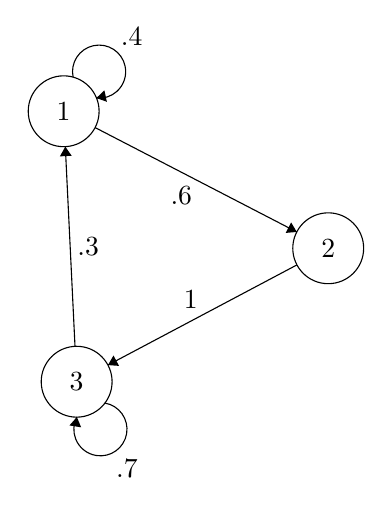
\begin{tikzpicture}[scale=0.15]
\tikzstyle{every node}+=[inner sep=0pt]
\draw [black] (19.3,-16.5) circle (3);
\draw (19.3,-16.5) node {$1$};
\draw [black] (41.7,-28.1) circle (3);
\draw (41.7,-28.1) node {$2$};
\draw [black] (20.4,-39.4) circle (3);
\draw (20.4,-39.4) node {$3$};
\draw [black] (21.96,-17.88) -- (39.04,-26.72);
\fill [black] (39.04,-26.72) -- (38.56,-25.91) -- (38.1,-26.8);
\draw (29.26,-22.8) node [below] {$.6$};
\draw [black] (20.101,-13.621) arc (192.17983:-95.82017:2.25);
\draw (25.06,-10.98) node [above] {$.4$};
\fill [black] (22.07,-15.38) -- (22.96,-15.7) -- (22.75,-14.73);
\draw [black] (39.05,-29.51) -- (23.05,-37.99);
\fill [black] (23.05,-37.99) -- (23.99,-38.06) -- (23.52,-37.18);
\draw (30.06,-33.25) node [above] {$1$};
\draw [black] (22.781,-41.205) arc (80.56505:-207.43495:2.25);
\draw (24.66,-45.94) node [below] {$.7$};
\fill [black] (20.42,-42.39) -- (19.79,-43.1) -- (20.78,-43.26);
\draw [black] (20.26,-36.4) -- (19.44,-19.5);
\fill [black] (19.44,-19.5) -- (18.98,-20.32) -- (19.98,-20.27);
\draw (20.42,-27.93) node [right] {$.3$};
\end{tikzpicture}
\end{center}
\item[\textbf{c. }] \textbf{(4 points)} It turned out that person 1 loved the movie, person 2 thought it was pretty good, and person 3 didn't get it: $p(0)=(1,0.7,0)$. Find $p(1)$ and $p(2)$. 
\item[\textbf{d. }] \textbf{(6 points)} What are the limiting opinions? In other words, find $\lim_{t\to\infty}p(t)$. Does the group reach a consensus? Give an intuitive explanation of why consensus is reached. 
\item[\textbf{e. }] \textbf{(7 points)} Give an example of a network with $n=3$ with no isolated nodes, and a vector of initial opinions, such that a consensus is never reached -- that is, so the sequence of vectors $(p(t))_{t=1}^\infty$ has no limit. 
\item[\textbf{f. }] \textbf{(7 points)} Suppose now agents are arranged in a ring, numbered $1,2,\ldots,n$ with person $i$ putting $1/2$ of her updating weight on himself ($m_{ii}=1/2$) and $1/2$ of her weight on his clockwise neighbor($m_{i,i+1}=1/2$). Indices are read modulo $n$.

 What will opinions converge to now? I.e., write down an explicit formula for $p(\infty)$, which is defined to be $\lim_{t \to \infty} p(t)$. This formula should involve only references to entries of $p(0)$ and $n$. This can be done with little calculation and largely through reasoning.
 
% \item[\textbf{g. }] \textbf{(5 points)} Continuing the setup of (f), suppose initial opinions $p_i(0)$ are drawn independently from a standard normal distribution. What is the standard deviation of $p_i(\infty)$ for a typical $i$? 

 \end{itemize}


\paragraph{5. Learning Influence Locally (again) (25 points)}
\par (If you don't like backstories in your psets, feel free to skip down a couple paragraphs. This problem is similar to problem 5 from problem set 6, but with a new diffusion model---something very similar to the Voter model.)
\par Raynor's been hired by a hot new social network called BetaPatch. They're not entirely sure what they do, but they know they only want the most popular, influential people using their app, so they'd like to figure that out who that is, and they want Raynor to take care of it.
\par Thanks to some lengthy field work on Facebook and a very divisive poll about local Mexican eateries in Harvard Square, Raynor has some data of the student network and how opinions change in the student community over time. He now wants to work backwards from this data using the Voter model as an assumption to derive popularity of students.
\par As in problem set 6, let's say we have a graph $G = (V,E)$ and some opinion data for each node $u \in V$. Assume each node (student) has an opinion that changes over time based on the influence of its neighbors (Instagram accounts) for a particular observed diffusion process (procrastination in the library). For a particular observed diffusion process $i$, let $opinion_i$ be a vector of timestamped opinions, where $opinion_i[u]$ is a vector such that $opinion_i[u][t]$ is equal to the opinion of node $u$ at time $t$ during observed cascade $i$, where $t$ ranges from $0$ to $\tau - 1$ so that $opinion_i[u]$ has length $\tau$, where opinions are either $0$ (node is inactive) or $1$ (active).
\par Our model is the same as the Voter model, but using a deterministic threshold rather than a probabilistic one. In this model, each directed edge $(u, v)$, has some corresponding edge weight $w_{(u,v)} \in (0,1]$. At each time step $t$, node $u$ will look at each of its neighbors and update its opinion to reflect the majority ``weighted" opinion---that is, if $\sum\limits_{v \in N(n)} w_{(u,v)}o_{t-1}(v) \ge .5$, then $u$ will update its opinion to be $1$ at time step $t$, and otherwise, will update its opinion to be $0$ at time step $t$, where $o_{t-1}(v)$ is the opinion of node $v$ at time step $t-1$ and is either $0$ or $1$. How can we help Raynor out by describing this situation using a linear program such that solving said linear program will give us an approximation for the edge weights? 
\par If we want to fit the Voter model locally to the opinion data, we can learn each of the edge weights $w_{(u,v)}$ in the graph by modeling the problem as binary classification and solving using a linear program. Consider a node $n$. We're trying to learn each of the edge weights $w_{(u,v)}$ for $v \in N(u)$. If we have some opinion data, and we know that at some time step $t$, $u$ has opinion $0$, and at time step $t+1$, $u$ has opinion $1$, we know that the sum of the edge weights to $u$'s neighbors that had opinion $0$ at $t-1$ was $\ge .5$ at $t-1$, but was $< .5$ at $t$.

\par The file $pset8\_network.txt$ is a directed graph, where $a \quad b$ corresponds to an edge from $a$ to $b$. The file $node\_opinions.pk$ is an array of opinions, where each entry $node\_opinions[i]$ is a dictionary equivalent to the vectors $opinion_i$ described above, such that $opinion_i[n]$ gives the vector of timestamped opinions described.

\begin{itemize}
\item[\textbf{a. }] \textbf{(1 point)} Load the file $pset8\_opinions.pk$. If you're using python, you can use python's `pickle` library and the `load` function to easily turn the file into an array; if you're using another language, we've provided $node\_opinions.json$, a JSON-encoded file that you can easily load in any language using the standard JSON encoding and the respective JSON library for your language (though you might have to do some additional string to integer conversion). What is $\tau$ and how many different diffusion processes are there? 
\item[\textbf{b. }] \textbf{(1 point)} Now load the file $pset8\_network.txt$. How many nodes are there? What is the average (out-)degree?
\item[\textbf{c. }] \textbf{(10 points)} Because he tends to have to debug a lot, Raynor first wants to make sure he has the right setup by writing down how influence will affect opinions. Using the definition of the Voter model described in lecture, and given a node $u$, write the linear program that, given $d$ diffusion processes with $\tau$ time steps each, uses all available information to approximate the edge weights $w_{(u,v)}$ for $v \in N(u)$. That is, write below the set of linear equations that constrain how a node in the voter model influences its neighbors.\\

Feel free to use indices to refer to time steps and cascades, but \textbf{be clear with all your notation and what means what.} (Raynor won't be able to read messy variables! It might even be helpful to describe what each individual equation refers to.) Don't forget to also include constraints such as the fact that all the edge weights have to be nonnegative, or that the weights for a single node should add up to one.

\item[\textbf{d. }] \textbf{(10 points)} Time for Raynor to get coding--or rather, for you to get coding. Using the linear program you described above, solve the program for each node and approximate the edge weights of each $e \in E$. Raynor is lazy, so to solve the program, you can use any one of the many linear program solver packages available (for python, scipy has a linear programming package).\\

Note that linear program solver packages will find variables that satisfy the constraints provided and fit some maximization or minimization constraint. \textbf{For the sake of making everything standardized for the grader, just maximize the sum of all the variables you're calculating in the linear program}. Additionally, since we know that the Voter model can be fit to the data (since the data was generated by the Voter model! Raynor's data is precise), we won't need to worry about slack variables. \\

What's the estimated weight of edge $(2,16)$? Of $(29, 22)$? Additionally, submit your estimates as a separate file formatted as a .csv, where entries in the first column correspond to the first node in the edge, entries in the second column correspond to the second node in the edge, and entries in the third column correspond to the edge weight.

\item[\textbf{e. }] \textbf{(3 points)} Assuming popularity is the average of influence, what five students (nodes) should Raynor first invite to the app and what's their average influence? You should use edge weights as measures of influence, but consider the Voter model and be careful about the direction of your edges!... 
\end{itemize}

\end{document}
